\section{Implementación Contenerizada con Docker}
	Se utilizó la siguiente declaración YAML docker-compose.yml para orquestar el levantamiento del servicio que contiene al motor de base de datos Oracle solicitado:

	\begin{lstlisting}[language=yaml, caption={Archivo docker-compose.yml para Oracle Database XE}]
		
		services:
		oracle-xe:
		image: container-registry.oracle.com/database/express:21.3.0-xe
		container_name: oracle21c-xe
		restart: unless-stopped
		ports:
		- "1521:1521"
		- "5500:5500"
		environment:
		- ORACLE_PWD=${ORACLE_PASSWORD}  # Cambia esto por una contraseña segura
		- ORACLE_CHARACTERSET=AL32UTF8
		volumes:
		- oracle_data:/opt/oracle/oradata
		shm_size: 2gb
		
		volumes:
		oracle_data:
		
	\end{lstlisting}
	
	El valor de contraseña \textbf{ORACLE\_PWD} esta parametrizado para ser leído mediante archivo de variables de entorno \textbf{.env}
	
	Se puede acceder al repositorio de esta evidencia mediante el siguiente enlace:
	
	\vspace{0.5cm}
	\begin{center}
		\href{https://github.com/jota2209/GA4-210602033-AA1-EV02}{→ Click aquí para ir a repositorio de GitHub ←}
		
	\end{center}
	\vspace{0.5cm}
	
	\subsection{Despliegue y Extinción de Contenedores y sus Servicios}
	Para levantar lo servicios se debe ejecutar en la terminal \textbf{docker compose up -d} para levantar los servicios, \textbf{docker compose down} para detenerlos (si se agrega el flag -v se eliminará el volumen que contiene la información de la base de datos) es decir \textbf{docker compose down -v}
	
	
	\subsection{Verificación de servicios corriendo}
	Esta labor se realiza mediante la ejecución de:
	
	\begin{lstlisting}[language=bash, caption={Comando para verificar contenedores corriendo desde la CLI}]
		docker ps	
	\end{lstlisting}
	
	\begin{figure}[htbp]
		\centering
		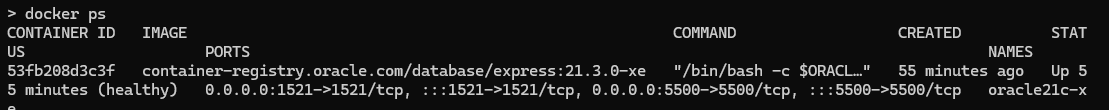
\includegraphics[width=1.0\textwidth]{../../images/dockerps_cli.png}
		\caption{Verificación de contenedores corriendo mediante terminal}
		\label{fig:Screenshot de contenedores corriendo mediante terminal}
	\end{figure}
	\FloatBarrier
	
	También podemos verificar mediante la interfaz de Docker Desktop
	
	\begin{figure}[htbp]
		\centering
		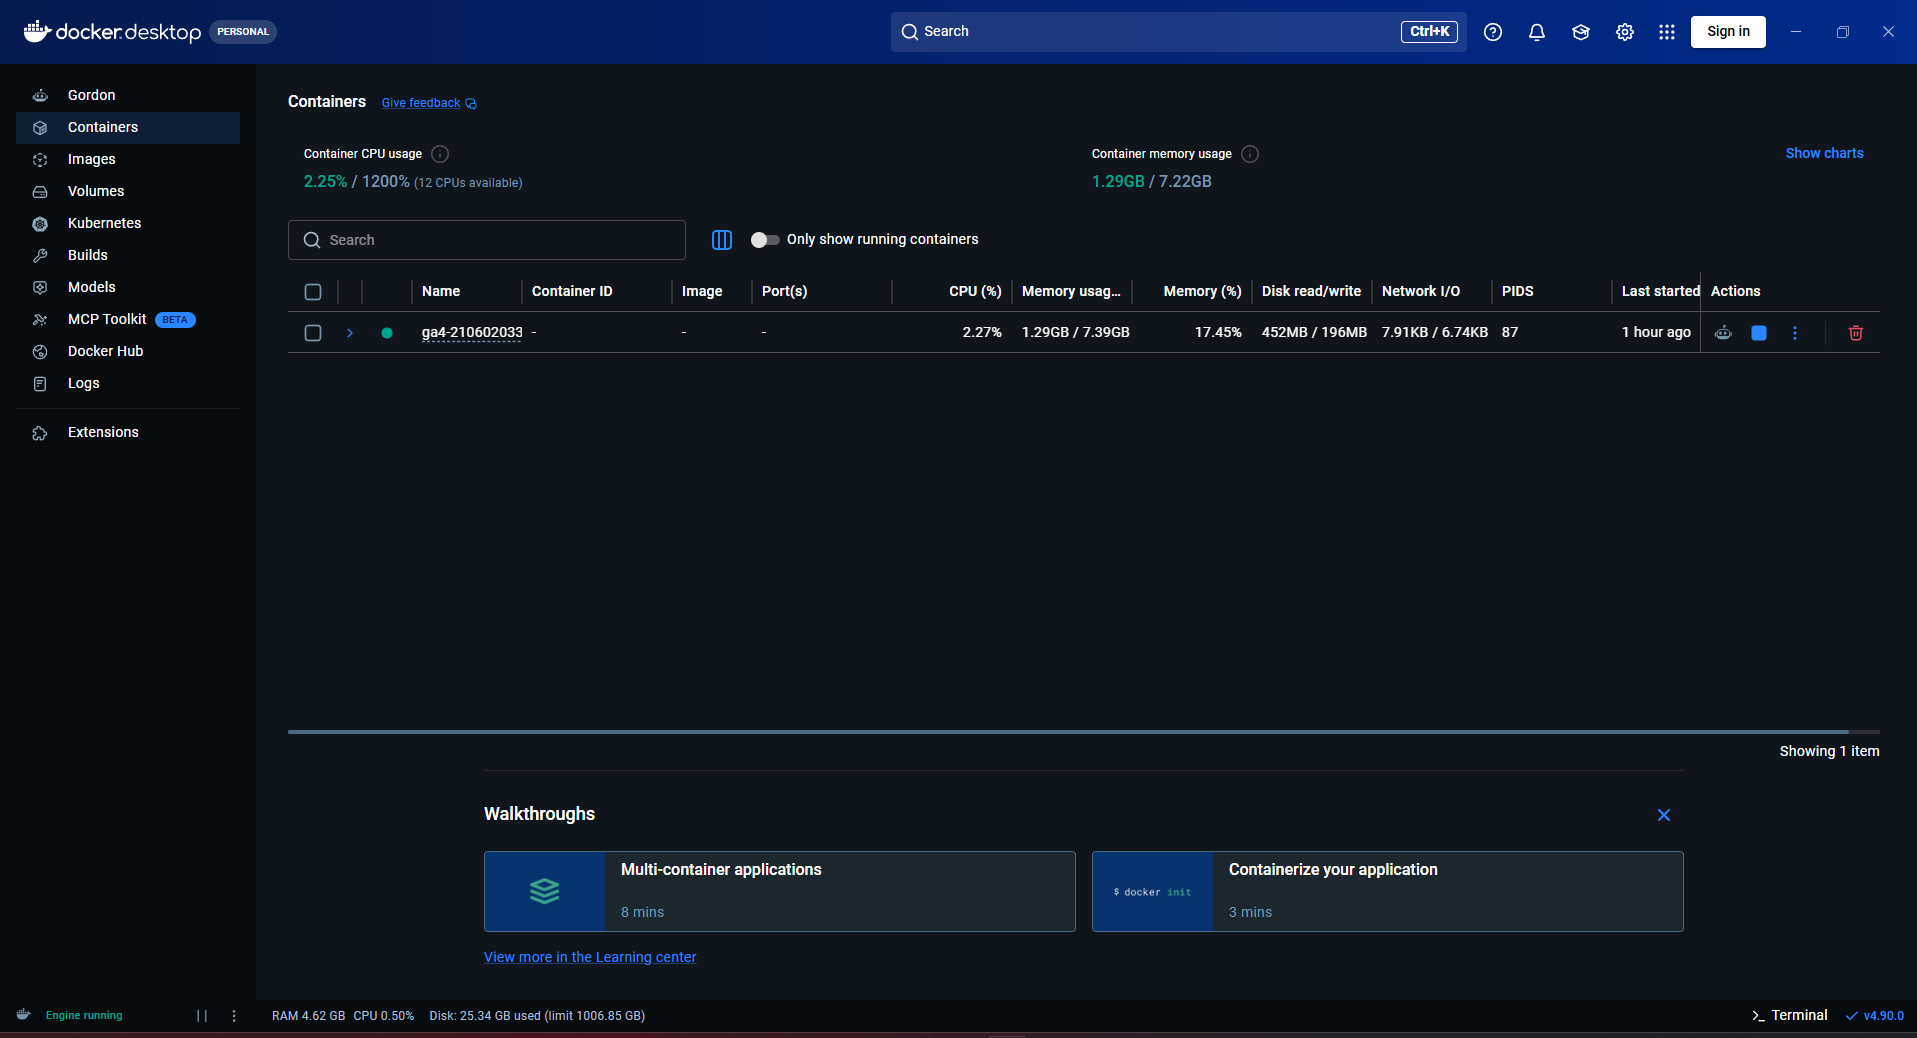
\includegraphics[width=1.0\textwidth]{../../images/docker_desktop.png}
		\caption{Verificación de contenedores corriendo mediante Docker Desktop}
		\label{fig:Screenshot Docker Desktop mostrando contenedor corriendo}
	\end{figure}
	\FloatBarrier
	
	\subsection{Prueba de Conexión con el Cliente GUI SQL Developer}
	Una vez que verifiquemos que el motor de base de datos ya está corriendo en nuestra infraestructura local con contenedores, procedemos a hacer una prueba de conexión con las credenciales pertinentes usando \textbf{SYS} como nombre de usuario y el valor de ORACLE\_PASSWORD indicado en el archivo \textbf{.env} al probar la conexión si nos da Estado: Correcto podemos proceder a conectar.
	
	\begin{figure}[htbp]
		\centering
		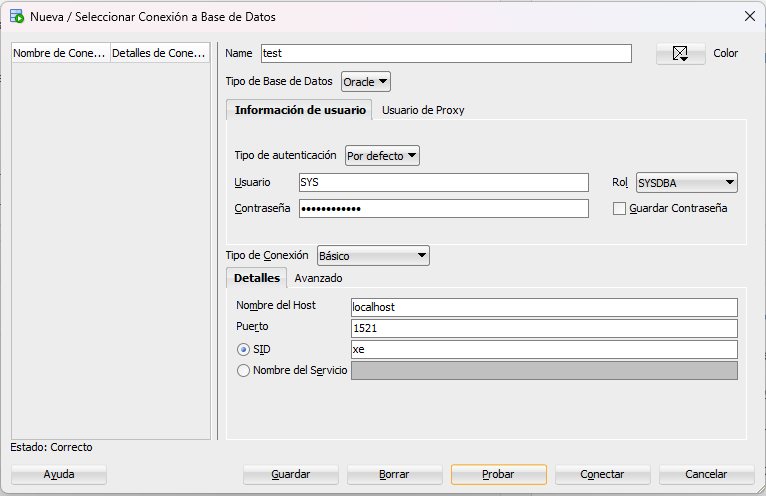
\includegraphics[width=1.0\textwidth]{../../images/success_conn01.png}
		\caption{Prueba de la conexión con estado correcto}
		\label{fig:Conexión en estado correcto}
	\end{figure}
	\FloatBarrier
	
	\begin{figure}[htbp]
		\centering
		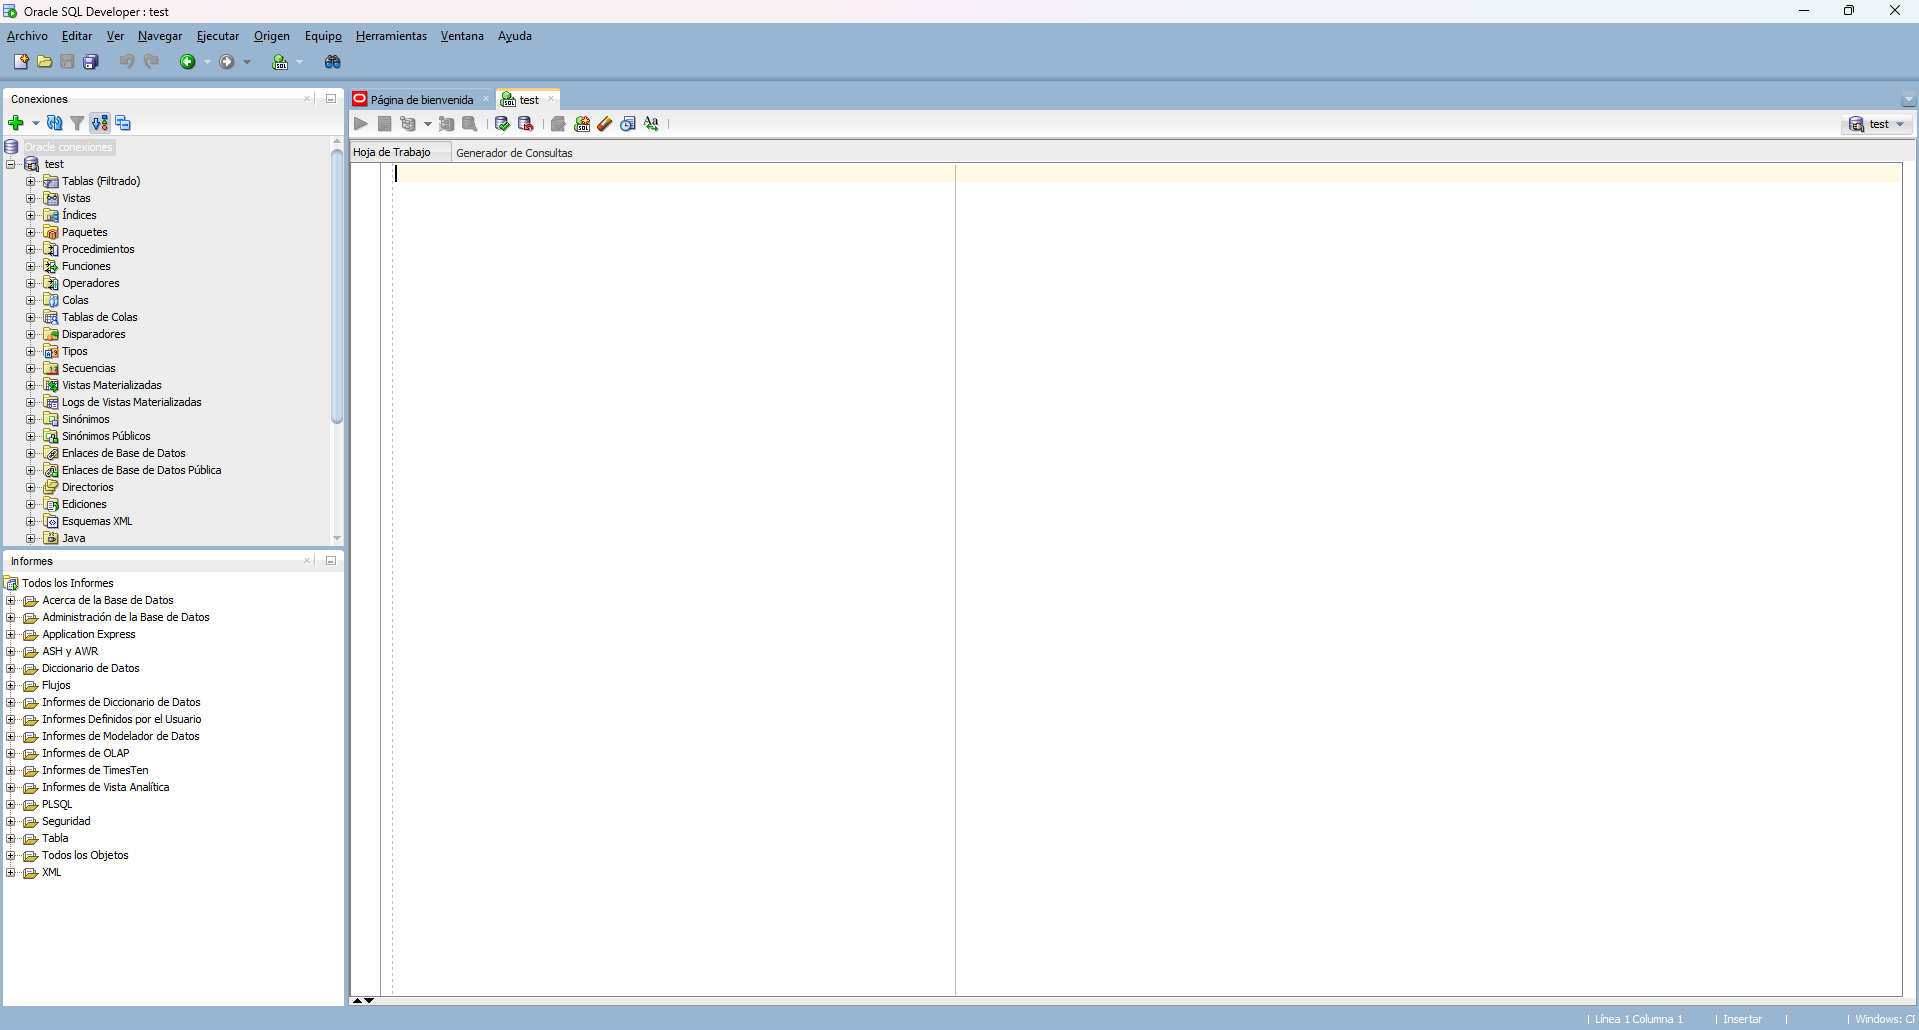
\includegraphics[width=1.0\textwidth]{../../images/success_conn02.png}
		\caption{Creación de Instancia de conexión "test"}
		\label{fig:Creación de instancia de conexión test}
	\end{figure}
	\FloatBarrier
	